\section{Troubleshooting}
If the application fails to start, the cause mainly is located in the generation or build process. Check the respective console for potential errors:

\subsection*{Generation error}
The \emph{eTrice C/Java Generator Console} outputs any errors, that were detected during generation, like model validation errors or missing imports/references.

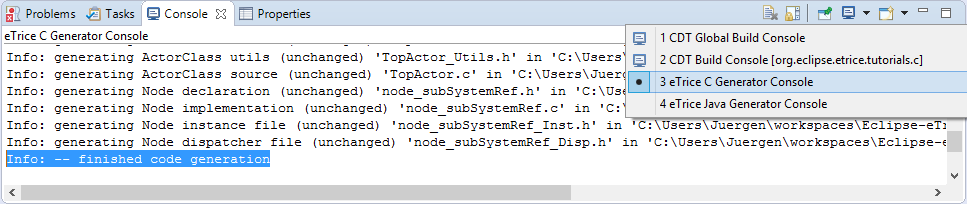
\includegraphics[width=\textwidth]{images/020-gen-console.png}


\subsection*{Build error}
The CDT Build Console outputs errors that occurred during the build process.

Common issues:
\begin{itemize}
	\item \emph{multiple main functions}: More than one executable application was built within a single project. Try a complete clean before rebuild of the project.
	\item compile error in generated user code: Check if the user code, that was generated out of the model causes compiler errors (e.g. state/transition action code or operation detail code). The default location for the generated code is the folder \emph{src-gen}.
\end{itemize}

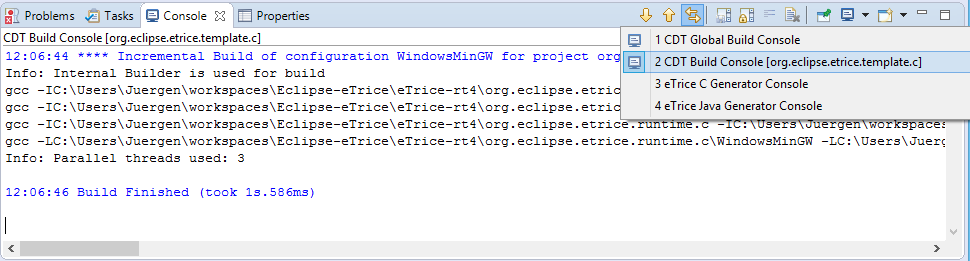
\includegraphics[width=\textwidth]{images/020-build-console.png}

\subsection*{Missing MSC}
The MSC is created when the application has been shutdown in proper form, thus has been terminated by typing \emph{quit} in the Console of the application. Depending on the Eclipse workspace settings, it might be necessary to refresh (F5) the \emph{log} folder manually.
